\documentclass[10pt, aspectratio=169]{beamer}
\usetheme{metropolis}

\usepackage[T1]{fontenc}
\usepackage[utf8]{inputenc}
\usepackage[spanish]{babel}
\usepackage{amsmath, amssymb}
\usepackage{booktabs}
\usepackage{lmodern}
\usepackage{graphicx}
\usepackage{svg}
\usepackage{xcolor}

\svgpath{{figs/}}

\metroset{block=fill}

% Accent palette matching the blue/red spin colors used throughout the plots
\definecolor{isingblue}{HTML}{378ADD}
\definecolor{isingred}{HTML}{D85A30}
\setbeamercolor{alerted text}{fg=isingred}
\setbeamercolor{progress bar}{fg=isingblue}
\setbeamercolor{title separator}{fg=isingblue}
\setbeamercolor{progress bar in head/foot}{fg=isingblue}
\setbeamercolor{progress bar in section page}{fg=isingblue}
\makeatletter
\setlength{\metropolis@titleseparator@linewidth}{1.3pt}
\makeatother
\setbeamerfont{title}{size=\LARGE,series=\bfseries}

% Three full-size slides, one per algorithm; the explanation goes in a
% text column next to the first (Metropolis) figure, at nearly full
% slide height. Glauber/Wolff are shown without comment.
\newcommand{\fullsizeslides}[3]{%
  \begin{frame}{#1 — Metropolis}
    \begin{columns}[c]
      \column{0.62\textwidth}
        \begin{center}\includesvg[height=0.78\textheight]{#2_Metropolis}\end{center}
      \column{0.38\textwidth}
        \small#3
    \end{columns}
  \end{frame}
  \begin{frame}{#1 — Glauber}
    \begin{center}\includesvg[height=0.82\textheight]{#2_Glauber}\end{center}
  \end{frame}
  \begin{frame}{#1 — Wolff}
    \begin{center}\includesvg[height=0.82\textheight]{#2_Wolff}\end{center}
  \end{frame}
}

\title{Algoritmos de simulación Montecarlo\\ en el modelo de Ising}
\author{Pablo López Serna \\ \footnotesize Tutor: Antonio González Sánchez}
\date{Julio 2026}
\institute{Trabajo de Fin de Grado\\Física}

\begin{document}

\maketitle

%-----------------------------------------------------------------------
\begin{frame}{Contenidos}
  \tableofcontents
\end{frame}

%=======================================================================
\section{Introducción y motivación}
%=======================================================================

\begin{frame}{El modelo de Ising}
  \begin{columns}
    \column{0.58\textwidth}
      \begin{itemize}
        \item Propuesto por Lenz (1920), resuelto en 1D por Ising (1925)
        \item Onsager (1944): solución exacta en 2D, con una fenomenología muy variada pese a sencillez
        \item Hamiltoniano para red cuadrada $L\times L$, sin campo externo:
          \[
            \mathcal{H} = -J\sum_{\langle i,j\rangle}\sigma_i\sigma_j, \quad \sigma_i = \pm 1
          \]
        \item Con $J = k_B = 1$, temperatura crítica exacta de Onsager:
          \[
            \boxed{T_c = \frac{2}{\ln(1+\sqrt{2})} \approx 2{,}2692}
          \]
      \end{itemize}
    \column{0.42\textwidth}
      \begin{center}
        
\includegraphics[width=\linewidth]{../article/fotos/2D_ising_model_on_lattice.svg.png}\\[0.4em]
        {\small Red cuadrada 2D: $\sigma_i=+1$ (rojo) y $\sigma_i=-1$ (azul)}
      \end{center}
  \end{columns}
\end{frame}

\begin{frame}{Objetivos}
  \begin{enumerate}
    \item Implementar y comparar tres algoritmos Montecarlo sobre el Ising 2D:
      \begin{itemize}
        \item \textbf{Metropolis}, \textbf{Glauber} (actualización local)
        \item \textbf{Wolff} (algoritmo de cúmulo)
      \end{itemize}
    \medskip
    \item Calcular los observables de equilibrio para $L\in\{16,32,64,128\}$:\quad
      $\langle|m|\rangle$,\; $c$,\; $\chi$,\; $U_4$,\; $\xi_L$
    \medskip
    \item Aplicar \textbf{escalado de tamaño finito (FSS)} para extraer exponentes críticos y $T_c$
    \medskip
    \item Comparar la \textbf{dinámica} de los tres algoritmos mediante el tiempo de autocorrelación integrado $\tau_{\text{int}}$
  \end{enumerate}
\end{frame}

%=======================================================================
\section{Fundamentos teóricos}
%=======================================================================

\begin{frame}{Transición de fase de segundo orden}
  \begin{itemize}
    \item En $T_c$ el parámetro de orden se anula de forma continua y la longitud de correlación diverge:
      \[ \xi \sim |t|^{-\nu}, \qquad t = \frac{T - T_c}{T_c} \]
    \item Los \textbf{exponentes críticos} $\nu,\gamma,\alpha,\beta,\ldots$ caracterizan completamente la transición
    \item Objetivo: medirlos numéricamente y contrastarlos con los valores exactos de Onsager
  \end{itemize}
\end{frame}

\begin{frame}{Transición de fase de segundo orden}
  \begin{figure}
    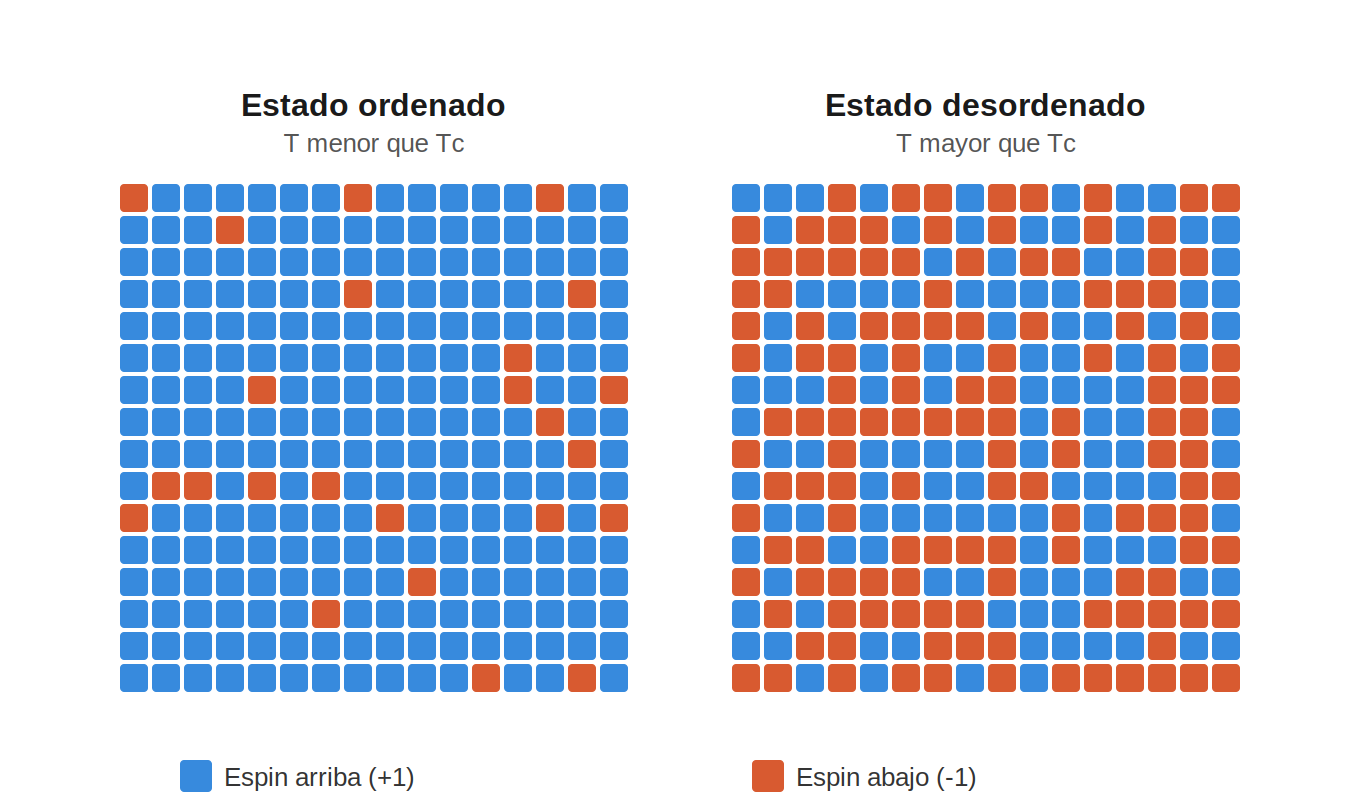
\includegraphics[width=0.7\textwidth]{figs/ising_estados.png}
  \end{figure}
\end{frame}

\begin{frame}{Observables del sistema}
  \begin{columns}
    \column{0.5\textwidth}
      \textbf{Magnetización} — parámetro de orden
      \[ \langle|m|\rangle = \frac{1}{N}\left\langle\left|\sum_i \sigma_i\right|\right\rangle \]

      \textbf{Capacidad calorífica} — fluctuaciones de $E$
      \[ c = \frac{\beta^2}{N}\!\left(\langle E^2\rangle - \langle E\rangle^2\right) \]

      \textbf{Susceptibilidad} — respuesta ante campo externo
      \[ \chi = \frac{L^2}{T}\!\left(\langle m^2\rangle - \langle|m|\rangle^2\right) \]

    \column{0.5\textwidth}
      \textbf{Cumulante de Binder} — adimensional, cruza en $T_c$
      \[ U_4 = 1 - \frac{\langle m^4\rangle}{3\langle m^2\rangle^2} \]
      $U_4\to 2/3$ (ordenado) \quad $U_4\to 0$ (desordenado)

      \medskip
      \textbf{Longitud de correlación} — del factor de estructura
      \[ \xi_L = \frac{1}{2\sin(\pi/L)}\sqrt{\frac{\chi(0)}{\chi(k_{\min})}-1} \]
  \end{columns}
\end{frame}

\begin{frame}{Escalado de tamaño finito (\textit{Finite Size Scaling})}
  \begin{itemize}
    \item \textbf{FSS:} En red finita, graficando las funciones $\xi_L$ y $\chi$ frente a $x=(T-T_c)L^{1/\nu}$ colapsan sobre una universal
    \item Las curvas de $U_4$ y $\xi_L/L$ se \textbf{cruzan en} $T_c$ para cualquier $L$
  \end{itemize}
\end{frame}

%=======================================================================
\section{Algoritmos Montecarlo}
%=======================================================================

\begin{frame}{Montecarlo: muestreo por importancia}
  \begin{itemize}
    \item La función de partición $Z = \sum_\sigma e^{-\beta\mathcal{H}(\sigma)}$ tiene $2^N$ términos $\Rightarrow$ inabarcable

    \medskip
    \item \textbf{Muestreo por importancia:} cadena de Markov que converge a la distribución de Boltzmann
    \[ P(\sigma) = \frac{e^{-\beta\mathcal{H}(\sigma)}}{Z} \]

    \item Condición suficiente: \textbf{balance detallado}
    \[ P(\sigma)\,W(\sigma\to\sigma') = P(\sigma')\,W(\sigma'\to\sigma) \]

    \item Los tres algoritmos difieren en la construcción de los movimientos $\sigma\to\sigma'$
  \end{itemize}
\end{frame}

\begin{frame}{Metropolis y Glauber}
  \begin{columns}[t]
    \column{0.5\textwidth}
      \textbf{Metropolis (1953)}
      \begin{enumerate}
        \item Elegir espín $i$ al azar
        \item Calcular $\Delta E$ al invertir $\sigma_i$
        \item Aceptar con probabilidad
          \[ W = \min\!\left(1,\, e^{-\beta\Delta E}\right) \]
      \end{enumerate}
      \begin{itemize}
        \item Sólo 5 valores posibles de $\Delta E$ en 2D $\Rightarrow$ probabilidades precalculables
      \end{itemize}

    \column{0.5\textwidth}
      \textbf{Glauber (1963)}
      \begin{enumerate}
        \item Elegir espín $i$ al azar
        \item Calcular $\Delta E$ al invertir $\sigma_i$
        \item Aceptar con probabilidad
          \[ W = \frac{1}{1+e^{\beta\Delta E}} \]
      \end{enumerate}
      \begin{itemize}
        \item Mismo exponente dinámico $z$ que Metropolis
        \item Probabilidad de aceptación sistemáticamente menor $\Rightarrow$ más lento
      \end{itemize}
  \end{columns}

  \medskip
  \textbf{1 paso Monte Carlo:} $N=L^2$ intentos de actualización de espín (un barrido completo de la red)
\end{frame}

\begin{frame}{Critical slowing down}
  \begin{itemize}
    \item El \textbf{tiempo de autocorrelación integrado} $\tau_{\text{int}}$ mide cuántos pasos MC hacen falta para obtener una configuración estadísticamente independiente
    \item Cerca de $T_c$ la longitud de correlación $\xi$ diverge, pero los algoritmos locales (Metropolis, Glauber) sólo invierten un espín por intento
    \item Decorrelar una región de tamaño $\xi$ requiere $\sim\xi^z$ pasos $\Rightarrow$ $\tau_{\text{int}}\sim L^z$ también diverge en $T_c$: es el \textbf{critical slowing down}
    \item Los algoritmos de cúmulo (Wolff) invierten regiones enteras a la vez $\Rightarrow$ $z\approx 0$, casi inmunes a este efecto
  \end{itemize}
\end{frame}

\begin{frame}{Wolff: algoritmo de cúmulo}
  \begin{columns}
    \column{0.55\textwidth}
      \begin{enumerate}
        \item Elegir espín semilla al azar
        \item Añadir vecinos con la misma orientación con probabilidad
          \[ p_{\text{add}} = 1 - e^{-2\beta J} \]
        \item Repetir recursivamente hasta completar el cúmulo
        \item Invertir \emph{todos} los espines del cúmulo
      \end{enumerate}

      \medskip
      \begin{block}{Ventaja clave}
        Cerca de $T_c$, el cúmulo abarca una fracción grande de la red $\Rightarrow$ \textbf{prácticamente elimina el critical slowing down}
      \end{block}

    \column{0.45\textwidth}
      \textbf{Exponente dinámico:}
      \begin{itemize}
        \item Metropolis/Glauber: $z \approx 2{,}17$
        \item Wolff: $z \approx 0{,}25$
      \end{itemize}

      \medskip
      \textbf{1 paso MC de Wolff:}\\
      suficientes cúmulos hasta girar $N$ espines en total (comparable a 1 barrido de red)
  \end{columns}
\end{frame}

%=======================================================================
\section{Configuración de la simulación}
%=======================================================================

\begin{frame}{Parámetros de la simulación}
  \begin{columns}
    \column{0.5\textwidth}
      \textbf{Tamaños simulados}
      \[ L \in \{16,\; 32,\; 64,\; 128\} \]
      Factor de variación $\times 8$ entre extremos

      \medskip
      \textbf{Arranque:} frío ($\sigma_i=+1$) para evitar metaestabilidad

      \medskip
      \textbf{Pasos de medida:} $N_{\text{steps}} = 1{,}99\times10^6$
      \begin{itemize}
        \item Metropolis/Glauber: muestra cada 50 pasos
        \item Wolff: muestra cada 5 pasos
      \end{itemize}

    \column{0.5\textwidth}
      \textbf{Malla de temperaturas adaptativa}
      \begin{itemize}
        \item Ventana fina: $[T_c - T_c/L,\; T_c + 3T_c/L]$ con $\Delta T = 0{,}1\,T_c/L$ (40 puntos)
        \item Rango grueso: $[0{,}15,\;5{,}0]$ con $\Delta T = 0{,}1$
      \end{itemize}

      \medskip
      {\small
      \begin{tabular}{cc}
        \toprule
        $L$ & Ventana fina \\
        \midrule
        16  & $[2{,}127,\;2{,}695]$ \\
        32  & $[2{,}198,\;2{,}482]$ \\
        64  & $[2{,}234,\;2{,}376]$ \\
        128 & $[2{,}251,\;2{,}322]$ \\
        \bottomrule
      \end{tabular}}
  \end{columns}
\end{frame}

%=======================================================================
\section{Resultados}
%=======================================================================

\fullsizeslides{Capacidad calorífica $c$}{c}{%
  \begin{itemize}
    \item El máximo se agudiza y desplaza hacia $T_c$ al crecer $L$
    \item Divergencia logarítmica ($\alpha=0$): extracción de $T_c$ poco precisa
    \item Los tres algoritmos dan resultados prácticamente idénticos
  \end{itemize}}

\fullsizeslides{Magnetización $\langle|m|\rangle$}{m}{%
  \begin{itemize}
    \item Parámetro de orden: $\to 1$ en la fase ordenada, $\to 0$ en la desordenada
    \item La caída se hace más abrupta al aumentar $L$, aproximándose al salto discontinuo del límite termodinámico
  \end{itemize}}

\fullsizeslides{Cumulante de Binder $U_4$}{fss_binder}{%
  \begin{itemize}
    \item Cociente adimensional de momentos de $m$: no depende de la normalización del observable
    \item Las curvas se cortan en $T_c$ con valor universal $U_4^*\approx 0{,}61$, coherente con Onsager
  \end{itemize}}

\begin{frame}{Extrapolación de $T_c$ con el cumulante de Binder}
  \begin{center}
    \includesvg[width=0.95\textwidth]{extrp_lin}
  \end{center}
  \vspace{-0.3em}
  \begin{itemize}
    \item Cruces de $U_4$ frente a $1/L^2$; ajuste lineal extrapola a $T_c$
    \item $T_c$ extrapolada: Metropolis $=2{,}2726$,\; Glauber $=2{,}2693$,\; Wolff $=2{,}2720$\quad (Onsager: $2{,}2692$)
    \item Solo Wolff muestra la mejora sistemática al crecer $L$; Metropolis/Glauber están dominados por ruido estadístico
  \end{itemize}
\end{frame}

\fullsizeslides{Susceptibilidad magnética $\chi$}{suscept}{%
  \begin{itemize}
    \item Mide la respuesta ante un campo externo mediante las fluctuaciones de $m$
    \item El pico diverge con $L$ siguiendo $\chi_{\max}\sim L^{\gamma/\nu}$
  \end{itemize}}

\begin{frame}{Escalado de $\chi_{\max}$ con $L$}
  \begin{center}
    \includesvg[width=0.95\textwidth]{chi_scaling}
  \end{center}
  \vspace{-0.3em}
  \begin{itemize}
    \item Pendiente en escala log-log $\approx 1{,}75$ (exacto: $\gamma/\nu = 7/4$)
  \end{itemize}
\end{frame}

\fullsizeslides{Colapso FSS de la susceptibilidad}{suscept_fss}{%
  \begin{itemize}
    \item Metropolis/Glauber: pico en $x\approx 1$;\quad Wolff: $x\approx 1{,}5$
    \item La diferencia se debe al \emph{critical slowing down}: medidas correlacionadas para $L$ grandes en los algoritmos locales
  \end{itemize}}

\fullsizeslides{Longitud de correlación $\xi_L$}{xi_vs_T}{%
  \begin{itemize}
    \item Se extrae del factor de estructura $S(k)$ mediante el estimador de Caracciolo–Sokal
    \item Los máximos crecen con $L$ y se desplazan hacia $T_c$
  \end{itemize}}

\fullsizeslides{Ratio $\xi_L/L$}{xi_ratio}{%
  \begin{itemize}
    \item Las curvas se cruzan en $T_c$, igual que el cumulante de Binder
    \item Observable completamente distinto: comprobación de coherencia interna sobre la estimación de $T_c$
  \end{itemize}}

\begin{frame}{Escalado de $\xi_L$ con $L$}
  \begin{center}
    \includesvg[width=0.95\textwidth]{xi_scaling}
  \end{center}
  \vspace{-0.3em}
  \begin{itemize}
    \item Pendiente $\approx 1$ $\Rightarrow$ $\nu \approx 1$
  \end{itemize}
\end{frame}

\fullsizeslides{Colapso FSS de $\xi_L/L$}{xi_fss}{%
  \begin{itemize}
    \item Variable de escala $x=(T-T_c)L^{1/\nu}$, sin ningún parámetro libre
    \item El colapso confirma $\nu=1$, en pleno acuerdo con el valor exacto de Onsager
  \end{itemize}}

%=======================================================================
\section{Comparativa dinámica}
%=======================================================================

\fullsizeslides{Tiempo de autocorrelación $\tau_{\text{int}}$}{tau_vs_T}{%
  \begin{itemize}
    \item Metropolis/Glauber: pico en $T_c$ que crece con $L$ (\emph{critical slowing down});\quad Glauber $\approx 1{,}5$–$2\times$ más lento
    \item Wolff: $\tau_{\text{int}}\sim\mathcal{O}(1)$ en todo el rango, sin estructura apreciable
  \end{itemize}}

\begin{frame}{Exponente dinámico $z$}
  \begin{center}
    \includesvg[width=0.95\textwidth]{tau_scaling}
  \end{center}
  \vspace{-0.3em}
  \begin{columns}
    \column{0.5\textwidth}
      $\tau_{\max}(L)\sim L^z$:
      \begin{itemize}
        \item Metropolis/Glauber: $z\approx 2$
        \item Wolff: $z\approx 0$
      \end{itemize}
    \column{0.5\textwidth}
      Consecuencia práctica para $L=128$:\\
      obtener una muestra independiente en $T_c$ cuesta $\sim L^2 \approx 16\,000$ veces más con algoritmos locales
  \end{columns}
\end{frame}

%=======================================================================
\section{Conclusiones}
%=======================================================================

\begin{frame}{Conclusiones}
  \begin{block}{Equilibrio}
    \begin{itemize}
      \item Los tres algoritmos reproducen correctamente la física de equilibrio
      \item $T_c$ estimada por cruces de $U_4$ es compatible con Onsager ($U_4^*\approx 0{,}61$)
      \item Exponentes $\gamma/\nu \approx 7/4$ y $\nu\approx 1$: datos en la clase de universalidad del Ising 2D
    \end{itemize}
  \end{block}

  \begin{block}{Dinámica}
    \begin{itemize}
      \item Metropolis y Glauber: $z\approx 2$; Glauber sistemáticamente $1{,}5$–$2\times$ más lento
      \item Wolff: $z\approx 0$, elimina prácticamente el \emph{critical slowing down}
      \item La correlación residual de Metropolis/Glauber degrada el colapso FSS para $L$ grandes
    \end{itemize}
  \end{block}

  \begin{block}{Perspectivas}
    Extensión al Ising 3D, donde no hay solución exacta y los exponentes solo se conocen numéricamente. Adición de estimadores de incertidumbre (bootstrap, jackknife).
  \end{block}
\end{frame}

\begin{frame}[standout]
  \Huge Gracias
\end{frame}

\end{document}
